%%==================================================
%% chapter01.tex for BIT Master Thesis
%% modified by yang yating
%% version: 0.1
%% last update: Dec 25th, 2016
%%==================================================
\chapter{相关工作}
\label{chap:intro}
\section{复杂网络}

随着近几年关于复杂网络(Complex network)理论及其应用研究的不断深入,已有大量关于复杂网络的文章发表在Science,RL,NAS等国际一流的刊物上,侧面反映了复杂网络已经成为物理界的一个新兴的研究热点。人们开始尝试应用这种新的理论工具来研究现实世界中的各种大型复杂系统,其中人们关注的热点问题是复杂系统的结构以及系统的结构与功能之间的关系。

在自然界中存在的大量复杂系统都可以通过形形色色的网络加以描述。一个典型的网络是由许多节点与节点之间的连边组成,其中节点用来代表真实系统中不同的个体,而边则用来表示个体间的关系,往往是两个节点之间具有某种特定的关系则连一条边,反之则不连边,有边相连的两个节点在网络中被看作是相邻的。例如,神经系统可以看作大量神经细胞通过神经纤维相互连接形成的网络;计算机网络可以看作是自主工作的计算机通过通信介质如光缆、双绞线、同轴电缆等相互连接形成的网络。类似的还有电力网络、社会关系网络、交通网络、调度网络等等。

复杂网络的研究由于其学科交叉性和复杂性的特点,涉及了众多学科的知识和理论基础,尤其是系统科学、统计物理、数学、计算机与信息科学等,常用的分析方法和工具包括图论、组合数学、矩阵理论、概率论、随机过程、优化理论和遗传算法等。复杂网络的主要研究方法都是基于图论的理论和方法开展的,并已经取得了可喜的成果。但近几年,统计物理的许多概念和方法也已成功地用于复杂网络的建模和计算,如统计力学、自组织理论、临界和相变理论、渗流理论等,如网络结构熵的概念,并用它来定量地度量复杂网络的“序”。复杂网络模型在很多科学领域都得到广泛的应用。

\section{社交网络}
%\label{sec:***} 可标注label

社交网络(Social network)就是复杂网络中的一种,是由许多节点以及节点间关系构成的一个网络结构。节点通常是指个人或组织。社交网络代表各种社会关系,经由这些社会关系,把从偶然相识的泛泛之交到紧密结合的家人关系的各种人们或组织串连起来。因此,社交网络也被称为社会关系网络。社交网络依赖于一种或多种关系而形成,如价值观、理想、观念、兴趣爱好、友谊、血缘关系、共同厌恶的事物、冲突或贸易。由此产生的网络结构往往是非常复杂的。

随着网络时代的来临,社交软件成为人们日常生活中必不可少的模块,社交网络也随之被作为当下流行的研究课题。社交网络是指人与人之间以某种关系建立的的社会网络结构,这种关系可以是兴趣爱好,朋友熟人,经贸交易等。将社会行动者视为节点,社会关系视为连线的边,从而构造出社交网络的拓扑模型。社交网络本着“节约社交成本,高效获取信息”的目的,依靠特定的功能诉求,将相应的用户人群集结在同一平台,从而实现社会关系网络化的延伸,跨越了时间地域等的限制。相对于传统网络,社交网络包含以下特性:

(1)以人为基点构建的关系型社会网络。社交网络以人为中心,着重强调人与人之间的关系。如兴趣类社交平台百度贴吧,贴吧通过社交网络的优势,使得拥有相同兴趣爱好的人聚集在一起,以兴趣建立用户之间的联系,构造庞大的主题社交平台。由于社交网络中人为基点的特性,现存的社交网络软件往往是以用户为中心来进行产品设计和组织管理。

(2)虚拟化社会关系,现实社交关系的延伸。社交网络是人们真实生活的虚拟映射,网络上的社交行为也是人们日常社交的一部分。社交网络以人为主题,每个用户有其对应的 id 账号,并围绕该账号展开一系列工作和生活相关的社交行为,形成相应的朋友圈,以此拓展现实社交行为。如生活类的社交软件微信,微信将现实生活中的人际交往以互联网形式呈现,每个用户通过自己的 id 账号管理着自己的社交圈,丰富了用户的社会交际。社交网络跨越了时间地域等的限制,为用户提供了便捷。

社交网络分析是用来查看节点、链接之间的社会关系的分析方式。节点是网络中的个人参与者,链接则是参与者之间的关系。节点之间可以有很多种链接。一些学术研究已经显示,社交网络在很多层面运作,从家庭到国家层面都有,并扮演着关键作用,决定问题如何得到解决,组织如何运行,并在某种程度上决定个人能否成功实现目标。

对于社交网络分析,社区发现是其中一个十分重要的问题研究方向,社区发现也可以被称为社区检测。对于所有社交网络中的节点,判断它隶属于哪一个社区,从而把有相似属性的节点划分到同一个集合,一个大的网格节点集合可以被划为多个不同大小包含不同节点的子集,这就是社区发现。独立的分析每个社区结构的特点,可以得到社区之间的不同之处,这样我们可以迅速简便的获得自己想要的信息。

\section{社区发现}
%\label{sec:features}

社区发现(community detection,也可以译作社区检测)是一个复杂而有意义的过程,它对研究复杂网络的特性具有重要作用。给定一个网络图,找出其社区结构的过程就叫做社区发现。近几年,发现及分析复杂网络中的社区结构得到了许多学者的关注,同时也出现了很多的社区发现算法。

\subsection{社区结构定义}
%\label{sec:requirements}
(1)一般社区结构定义

目前对网络社区的定义还没有一个统一的标准,人们从不同的角度给出了不同的社区结构的定义。典型的包括:基于子图的局部定义和基于节点相似度的定义。

基于子图的局部定义:社区结构可以被看成网络拓扑结构中具有高内聚特点的若干节点集合,这些节点集合往往是某种具有独立功能或者性质的相对独立组件的抽象。因此,可以根据网络局部拓扑结构特点来定义社区结构。当前,被各领域学者广泛接受的一个描述定义是基于子图的局部定义。即社区结构是复杂网络节点集合的若干子集,每个子集之间的节点之间连接非常紧密,不同子集的节点之间连接比较稀疏,如图\ref{fig:fig2-1}所示。图中的网络由20个节点组成,这20个节点被划分成了三个社区结构,分别对应着图中的三个虚线内部的结构。

\begin{figure}
  \centering
  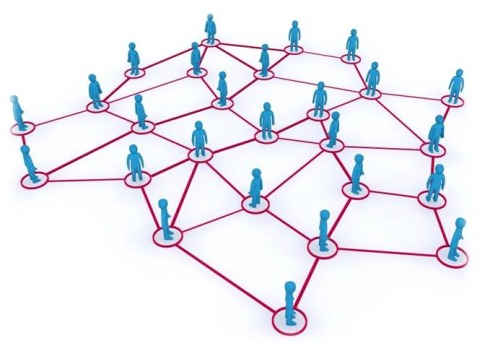
\includegraphics[width=0.75\textwidth]{figures/fig2-1}
  \caption{一个具有社区结构的网络示意图}
  \label{fig:fig2-1}
\end{figure}

 基于节点相似度的定义:从物理意义上讲,社区往往代表了复杂系统或者复杂网络中的具有相似或者相同功能的元素集合,这些元素相互协作或者相互作用,共同完成整个系统中某些相对独立的功能或者组织结构。据此,可以基于节点的相似度来定义社区,该定义假定社区内部节点都是相似的,社区间的节点相似性低,采用某种指标来衡量网络节点间的相似性,根据节点之间的相似性来定义社区结构。总体而言,从本质内涵来看,已有的社区结构的定义都是一致的,是由网络中所有个体组成的集合的子集,该集合中的个体基于某种属性连接紧密并和子集外的个体连接稀疏。但是紧密和稀疏并没有一个可以定量分析的标准,这些定义就没有多少实用的价值。

 (2)重叠社区结构定义

	在真实世界的社交网络中,社区结构呈现复杂多样的特点,大部分社区结构是重叠的,这就是说网络的节点集合中存在一些同时属于多个社区的节点,即重叠节点。比如,在社交网络中一个个体可以同时属于多个社会团体,各个组织之间有一些共有的个体。在各种类型的网络中,重叠节点一般十分重要。所以,网络中的重叠社区发现获得了越来越多人的关注。
  
  通常,重叠社区结构大致被分为两种类型:离散重叠社区和模糊重叠社区。对于前者,我们只要判断一个节点属不属于一个社区,也就是说节点要么属于一个社区,要么不属于这个社区。相反,模糊重叠需要计算节点对于不同的社区的隶属度,对于某个社区的隶属度有高有低。

\subsection{社区网络模型描述}

网络中社区结构表示的是网络中节点集合的子集。一般情况下,一个复杂的网络可以这样表示:由顶点集 $V$和边集 $E$组成的图$G=(V,E)$。节点个数表示为$n=|V|$,边数表示为$m=|E|$。如果任意两个节点对 $(i, j)$ 与 $(j, i)$表示的是同一条边,该图被称为无向图,否则,该被称为有向图。如果我们给图中的每一条边都设置一个代表关系强弱程度的数值,我们把这种图定义为有权图;否则,该图被称为无权图。显然,我们也可以把无权图看成图中每条边权重值都相同的有权图,比如权值都为1。在无向图中的定义中,节点i的度指的是以i为顶点的边的数目,记为,是所有含有该节点的边的数量的总和。在有向图的定义中,节点的度分为两种类型,入度和出度。以该节点为终点的边的数量为该节点的出入度,以该节点为起点的边的数量为该节点的出度。在无向图中无出入度之分。此外,我们还可以用邻接矩阵或者邻接表来表示网络的真实拓扑结构,邻接矩阵如果是对称矩阵那么表示的是无向图,如果是非对称的矩阵表示就是有向图。

\section{社区结构评价指标}

迄今为止,出现了各种各样的社区发现算法,如何评价不同的的发现算法的好坏是一个非常重要的问题。为此,学者们提出了多种社区结构评价指标用来评价网络社区划分质量,其中比较有代表性的有模块度、NMI等。下面详细介绍这些指标。

\subsection{模块度}

模块度是目前学者们最常用和经典的网络社区结构评价指标,它最初是被Newman等人于2004年提出来的\cite{2002Community}。其通过比较现有网络和基准网络在相同社区划分下的连接密度差来衡量网络社区的优劣,其中基准网络是由原网络具有相同度序列的随机网络。模块度计算公式如下:

\begin{equation}
  \label{eqn:LBmodel}
  Q=\frac{1}{2m}\sum_{i,j}\left [ A_{ij}-\frac{k_ik_j}{2m} \right ]\delta (c_i, c_j)  
\end{equation}

其中,A 表示网络中的邻接矩阵, m 表示网络中边的总数,$k_i$和$k_j$表示节点 i 和 j 的度数,$c_i$和$c_j$表示节点 i 和 j 所属的社区。如果$i=j,\delta(c_i,c_j)=1$,反之$\delta(c_i,c_j)=0$

......

\subsection{NMI}

随着在线社交网络的发展,人们发现在线社交网络的很多数据中存在着暗示各个节点的社区属性信息。例如,在人人网的学校信息便揭示了网络节点中属于同一学校的社区结构,Facebook中的兴趣信息同样表征了具有相同兴趣的虚拟用户群体。这些数据在为社区发现问题提供了丰富的信息的同时,也在一定程度上为虚拟社区结构优劣的评判提供了标准答案。针对这种预先拥有一定虚拟社区结构信息的情况下,Leon Danon等人【34】提出了Normalized Mutual Information(NMI)利用信息化熵来衡量算法划分的社区结构和预先已知的社区结构之间的差异。NMI是基于混合矩阵(Confusion Matrix)N来计算的数字指标。NMI公式如下:

\begin{equation}
  \label{eqn:LBmodel}
  NMI=\frac{ -2 \sum_{i,j} N_{ij}  ln{\frac{N_{ij}}{N_iN_j}} } {\sum_{i}N_iln{\frac{N_i}{n}}+\sum_{j}N_jln{\frac{N_j}{n}}}
\end{equation}

使用该数字指标,可以衡量划分出来的社区结构与已知的网络社区结构的差异程度值,该值越大,则表明获得的社区结构划分越好,当该值达到最大化值1时,说明算法发现的社区结构与已知社区结构完全已知,效果最好。

\begin{figure}
  \centering
  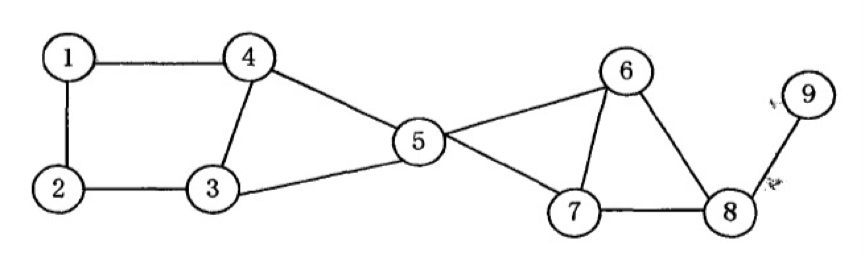
\includegraphics[width=0.75\textwidth]{figures/fig2-2}
  \caption{网络示例}\label{fig:fig2-2}
\end{figure}

下面以图\ref{fig:fig2-2}为例来说明计算NMI的过程。假设已知的最佳社区结构划分为集合{1,2,3,4}和{5,6,7,8},相应的社区划分向量表示为a = (1,1,1,1,2,3,3,3,3),再假设某算法获得的社区划分结构可以用向量表示为b = (3,3,3,3,2,1,1,1,1)来表示。根据已知的社区划分向量,可以构造混合矩阵N:

\begin{equation}
  \label{eqn:LBmodel}
  N=\begin{bmatrix}
    0 & 0 &4 \\ 
    0 & 1 & 0\\ 
    4 & 0 & 0
    \end{bmatrix}
\end{equation}

根据上式计算可知,该划分的NMI值为1。
